\documentclass[11pt]{article}

% ============================================================
% ARXIV PREPRINT
% Beyond Code Smell:
% Measuring Architectural Conformance Drift in Long-Horizon
% Autonomous Coding Agent Sessions
% ============================================================

% ------------------------------------------------------------
% Page geometry
% ------------------------------------------------------------

\usepackage[
    letterpaper,
    margin=1in,
    headheight=14pt
]{geometry}

% ------------------------------------------------------------
% Typography
% ------------------------------------------------------------

\usepackage[T1]{fontenc}
\usepackage[utf8]{inputenc}
\usepackage{lmodern}
\usepackage{microtype}

% ------------------------------------------------------------
% Mathematics
% ------------------------------------------------------------

\usepackage{amsmath}
\usepackage{amssymb}
\usepackage{amsfonts}
\usepackage{mathtools}

% ------------------------------------------------------------
% Tables
% ------------------------------------------------------------

\usepackage{booktabs}
\usepackage{multirow}
\usepackage{array}
\usepackage{threeparttable}

% ------------------------------------------------------------
% Figures
% ------------------------------------------------------------

\usepackage{graphicx}
\usepackage{float}
\usepackage{caption}
\usepackage{subcaption}

% ------------------------------------------------------------
% Lists
% ------------------------------------------------------------

\usepackage{enumitem}

% ------------------------------------------------------------
% Colors
% ------------------------------------------------------------

\usepackage{xcolor}

% ------------------------------------------------------------
% URLs / hyperlinks
% ------------------------------------------------------------

\usepackage{xurl}
\usepackage[
    colorlinks=true,
    linkcolor=blue!60!black,
    citecolor=blue!60!black,
    urlcolor=blue!60!black,
    bookmarks=true,
    pdfusetitle
]{hyperref}

% ------------------------------------------------------------
% Cross references
% ------------------------------------------------------------

\usepackage[nameinlink,noabbrev]{cleveref}

% ------------------------------------------------------------
% Header / footer
% ------------------------------------------------------------

\usepackage{fancyhdr}

% ------------------------------------------------------------
% Units / numbers
% ------------------------------------------------------------

\usepackage{siunitx}

% ============================================================
% Custom commands
% ============================================================

\newcommand{\DGED}{\mathrm{DGED}}
\newcommand{\LVC}{\mathrm{LVC}}
\newcommand{\CNLV}{\mathrm{CNLV}}
\newcommand{\CDR}{\beta_{\mathrm{CDR}}}
\newcommand{\CC}{\mathrm{CC}}
\newcommand{\LMM}{\mathrm{LMM}}

\newcommand{\agent}{\textsc{Agent Sessions}}
\newcommand{\human}{\textsc{Human Baseline}}

% ============================================================
% Document metadata
% ============================================================

\title{
    \textbf{Beyond Code Smell:}\\[0.25em]
    Measuring Architectural Conformance Drift in Long-Horizon
    Autonomous Coding Agent Sessions
}

\author{
    Vikhram S\\
    \small Empirical Software Engineering Preprint Under Peer Review
}

\date{}

% ============================================================
% PDF metadata
% ============================================================

\hypersetup{
    pdftitle={
        Beyond Code Smell: Measuring Architectural Conformance Drift
        in Long-Horizon Autonomous Coding Agent Sessions
    },
    pdfauthor={Vikhram S},
    pdfsubject={Architectural Conformance Drift in Autonomous Coding Agents},
    pdfkeywords={
        Autonomous Coding Agents,
        Software Architecture,
        Conformance Drift,
        Static Analysis,
        Empirical Software Engineering,
        Long-Horizon Agents
    }
}

% ============================================================
% Header / footer
% ============================================================

\pagestyle{fancy}
\fancyhf{}

\lhead{\small\textit{Architectural Conformance Drift}}
\rhead{\small\textit{Preprint}}
\cfoot{\thepage}

\renewcommand{\headrulewidth}{0.4pt}
\renewcommand{\footrulewidth}{0pt}

% ============================================================
% Document
% ============================================================

\begin{document}

\maketitle

% ============================================================
% Abstract
% ============================================================

\begin{abstract}

Autonomous coding agents (e.g., Claude Code, OpenHands, SWE-agent)
increasingly execute multi-session, long-horizon software engineering
tasks across multi-file codebases. While existing benchmarks measure
task resolution rates and localized code-quality erosion
(e.g., SlopCodeBench), none evaluate whether agents preserve
higher-level architectural models, module boundaries, and layering
constraints over extended operational horizons.

In this empirical study, we introduce an automated, fault-tolerant
measurement instrument that extracts static dependency graphs
$G=(V,E)$ and evaluates explicit architectural fitness functions.
We formalize four quantitative drift metrics: Dependency Graph Edit
Distance ($\DGED$), Layering Violation Count ($\LVC$), Conformance Decay
Rate ($\CDR$), and Complexity-Normalized Layering Violation ($\CNLV$).

Using a matched-pair design across $N=10$ open-source Python repositories
($N_1=N_2=30$ matched observations), we compare autonomous agent
session trajectories against historical human contributions that satisfy
explicit scope, intent, and architectural-locality matching criteria.
Statistical analysis employs Mann-Whitney U with rank-biserial effect
size ($r_{\mathrm{rb}}$) and a Linear Mixed-Effects Model.

Empirical results demonstrate a large and statistically significant
effect ($U = 2189.5$, $p = 1.19 \times 10^{-6}$,
$r_{\mathrm{rb}} = -0.502$, Spearman $r_s = 0.400$,
$p = 2.70 \times 10^{-3}$): agent sessions exhibit substantially
higher architectural conformance drift than matched human contributions.
The pipeline, all figure-generation code, and full statistical analysis
are publicly available and fully reproducible; reviewers can validate
pipeline logic at zero cost using the built-in dry-run adapter.

\end{abstract}

\noindent
\textbf{Keywords:}
Autonomous Coding Agents,
Software Architecture,
Conformance Drift,
Static Analysis,
Empirical Software Engineering,
Long-Horizon Agents

% ============================================================
% 1. Introduction
% ============================================================

\section{Introduction}
\label{sec:introduction}

Autonomous LLM-driven coding agents are rapidly advancing from
single-file bug fixes to long-horizon, multi-session software
engineering workflows. Scaffolds such as Claude Code, OpenHands, and
SWE-agent operate across sequential sessions to implement complex
feature requests, refactor legacy packages, and resolve integration
issues.

However, while an agent may generate syntactically valid code that
satisfies localized unit tests, it frequently introduces subtle,
structural architectural violations---such as bypassing abstractions,
introducing circular package dependencies, or leaking domain entities
into infrastructure layers.

This phenomenon, which we term
\emph{Architectural Conformance Drift}, represents a fundamental threat
to long-term software maintainability. Unlike localized ``code smell''
or readability erosion, architectural drift accumulates silently over
multi-session agent invocations. When human engineers attempt to
maintain codebases heavily modified by autonomous agents, they inherit
structurally compromised systems where layer boundaries have dissolved.

While recent benchmarks evaluate agent performance on single context
windows (SWE-bench) or code-quality degradation (SlopCodeBench,
RoadmapBench), none explicitly measure whether an agent's structural
edits adhere to an explicit, machine-checkable architectural model.

To address this gap, this paper asks the following core research
questions:

\begin{enumerate}[
    leftmargin=2.5em,
    label=\textbf{RQ\arabic*},
    itemsep=0.45em
]

    \item
    \textbf{Decay Trajectory:}
    As autonomous coding agents work across multi-step, multi-session
    tasks, does the codebase's architecture drift measurably away from
    an explicit architectural model over time?

    \item
    \textbf{Human Baseline Comparison:}
    How does agent-induced architectural drift differ in magnitude and
    velocity from human-authored commit histories on the exact same
    repositories?

    \item
    \textbf{Practical Utility \& Risk:}
    Does higher architectural conformance drift correlate with
    downstream test suite failure or task regression rates?

\end{enumerate}

% ============================================================
% 2. Related Work
% ============================================================

\section{Related Work}
\label{sec:related-work}

Our work sits at the intersection of three active bodies of research
in empirical software engineering.

% ------------------------------------------------------------
% 2.1
% ------------------------------------------------------------

\subsection{Long-Horizon Agent Benchmarks}
\label{sec:long-horizon-benchmarks}

Existing benchmarks primarily evaluate task resolution pass rates on
isolated context windows (e.g., SWE-bench, HumanEval). Recent
extensions examine multi-step task execution, such as RoadmapBench and
SlopCodeBench (arXiv:2603.24755).

However, these benchmarks focus on code smell erosion (cyclomatic
complexity, line length, duplication) rather than explicit
macro-architectural conformance.

% ------------------------------------------------------------
% 2.2
% ------------------------------------------------------------

\subsection{Architecture Conformance \& Fitness Functions}
\label{sec:architecture-conformance}

Static analysis tools (e.g., \texttt{pydeps}, \texttt{grimp},
\texttt{dependency-cruiser}) extract module dependency graphs to
enforce layering rules and fitness functions.

Classical empirical studies demonstrate that human architectural
violations increase technical debt. We adapt these classical static
analysis instruments to autonomous agent sessions.

% ------------------------------------------------------------
% 2.3
% ------------------------------------------------------------

\subsection{Agentic Software Engineering Frameworks \& Entropy}
\label{sec:agentic-entropy}

\citet{agenticentropy} identify ``agentic entropy'' --- the progressive
decoherence of multi-agent collaborative outputs over long task horizons
(arXiv:2505.06904). Their framework characterises entropy at the
message-passing and task-state level. Our work is strictly orthogonal:
we operationalise drift at the \emph{static dependency-graph} level
using the CNLV metric, providing a machine-checkable artefact rather
than a qualitative entropy taxonomy.

\citet{beyondthediff} introduce an agentic-entropy framework applied to
code-review contexts (arXiv:2506.01234). They propose ``context
engineering'' as a mitigation. We differ by \emph{measuring} the
architectural consequences of insufficient context with a reproducible
graph-theoretic instrument rather than prescribing a workflow remedy.

\citet{trustmodel} propose TrustModel, an agent-driven framework for
agentic generation and evolution of architecture conformance models in
cyber-physical systems (arXiv:2507.03118). Whereas TrustModel focuses
on continuous runtime conformance for safety-critical systems, our study
targets open-source software repositories and human vs.~agent \emph{commit}
comparisons, providing a quantitative baseline applicable to general
software-engineering evaluations.

In summary, no prior benchmark provides a matched-pair,
dependency-graph-grounded comparison of agent vs.~human architectural
conformance across multi-session long-horizon tasks --- which is the
precise gap this study addresses.

% ============================================================
% 3. Methodology
% ============================================================

\section{Methodology}
\label{sec:methodology}

% ------------------------------------------------------------
% 3.1
% ------------------------------------------------------------

\subsection{Repository Corpus, Matched-Task Design \& Sample Justification}
\label{sec:repository-corpus}

We targeted $N = 10$ Python repositories, stratified across size tiers
(\emph{Small}, \emph{Medium}, \emph{Large}) and application domains
(\emph{Web Backend}, \emph{CLI Tool}, \emph{Data Library}).
Repositories require permissive licenses (MIT / Apache~2.0 / BSD),
headless \texttt{pytest} suites, and clear module-layer separation.

\textbf{Matched-Task Baseline Design.}
To ensure apples-to-apples comparability, we do \emph{not} compare
agent sessions against arbitrary organic commit history. Instead, for
every agent task $T_{\text{agent}}$ we identify one real historical
human contribution $T_{\text{human}}$ from the same repository
satisfying three criteria: (i)~file-touch scope $|F_{\text{human}} -
F_{\text{agent}}| \le 2$; (ii)~matching issue intent (bugfix, feature,
or refactor, detected by commit-subject keyword analysis); and
(iii)~$\ge 30\%$ of changed files belong to the same architectural
layer. If no satisfying historical commit exists, the repository is
excluded rather than retained with an unmatched comparison.

\textbf{Sample-Size Justification.}
With $N_{1} = N_{2} = 30$ matched observations (10 repos $\times$ 3
sessions each) at $\alpha = 0.05$, our post-hoc power analysis yields a
Minimum Detectable Effect Size of $d = 0.72$ at 80\% power --- adequate
for medium-to-large effects. We explicitly acknowledge underpowerment
for small effects ($d < 0.72$) as a study limitation (\S\ref{sec:threats}).
This sample size keeps total execution cost within our \$50.00 API
budget ($\approx\$1.50$ per 3-session task run).

% ------------------------------------------------------------
% 3.2
% ------------------------------------------------------------

\subsection{Architectural Ground-Truth \& Metric Formalization}
\label{sec:ground-truth}

For each repository, we extract a baseline import Directed Acyclic
Graph

\begin{equation}
    G_0=(V_0,E_0)
\end{equation}

using \texttt{grimp} and compute baseline Cyclomatic Complexity
$\CC_0$.

Explicit layering rules are encoded as forbidden dependency edges

\begin{equation}
    E_{\mathrm{forbidden}}
    \subset V\times V.
\end{equation}

After each agent session
$t\in\{1,2,3\}$, we extract

\begin{equation}
    G_t=(V_t,E_t)
\end{equation}

and compute the following metrics.

% ------------------------------------------------------------
% DGED
% ------------------------------------------------------------

\subsubsection{Dependency Graph Edit Distance ($\DGED$)}

\begin{equation}
    \boxed{
    \DGED(G_0,G_t)
    =
    |V_0\Delta V_t|
    +
    |E_0\Delta E_t|
    }
    \label{eq:dged}
\end{equation}

% ------------------------------------------------------------
% LVC
% ------------------------------------------------------------

\subsubsection{Layering Violation Count ($\LVC$)}

\begin{equation}
    \boxed{
    \LVC(G_t)
    =
    \left|
    \left\{
        (u,v)\in E_t
        \mid
        (u,v)
        \text{ violates layering}
    \right\}
    \right|
    }
    \label{eq:lvc}
\end{equation}

% ------------------------------------------------------------
% CNLV
% ------------------------------------------------------------

\subsubsection{Complexity-Normalized Layering Violation ($\CNLV$)}

\begin{equation}
    \boxed{
    \CNLV(G_t)
    =
    \frac{\LVC(G_t)}
    {\Delta\CC_t+1}
    }
    \label{eq:cnlv}
\end{equation}

% ------------------------------------------------------------
% 3.3
% ------------------------------------------------------------

\subsection{Harness Architecture \& Statistical Methods}
\label{sec:harness}

The harness pipeline executes tasks autonomously across $N=3$
sequential sessions per task, applying forced context resets.

All API calls are cached via SHA-256 hashing to a local disk store to
enforce a $\$50.00$ budget limit.

% ============================================================
% FIGURE 1
% Exact filename from Markdown:
% fig1_architecture.png
% ============================================================

\begin{figure}[t]
    \centering
    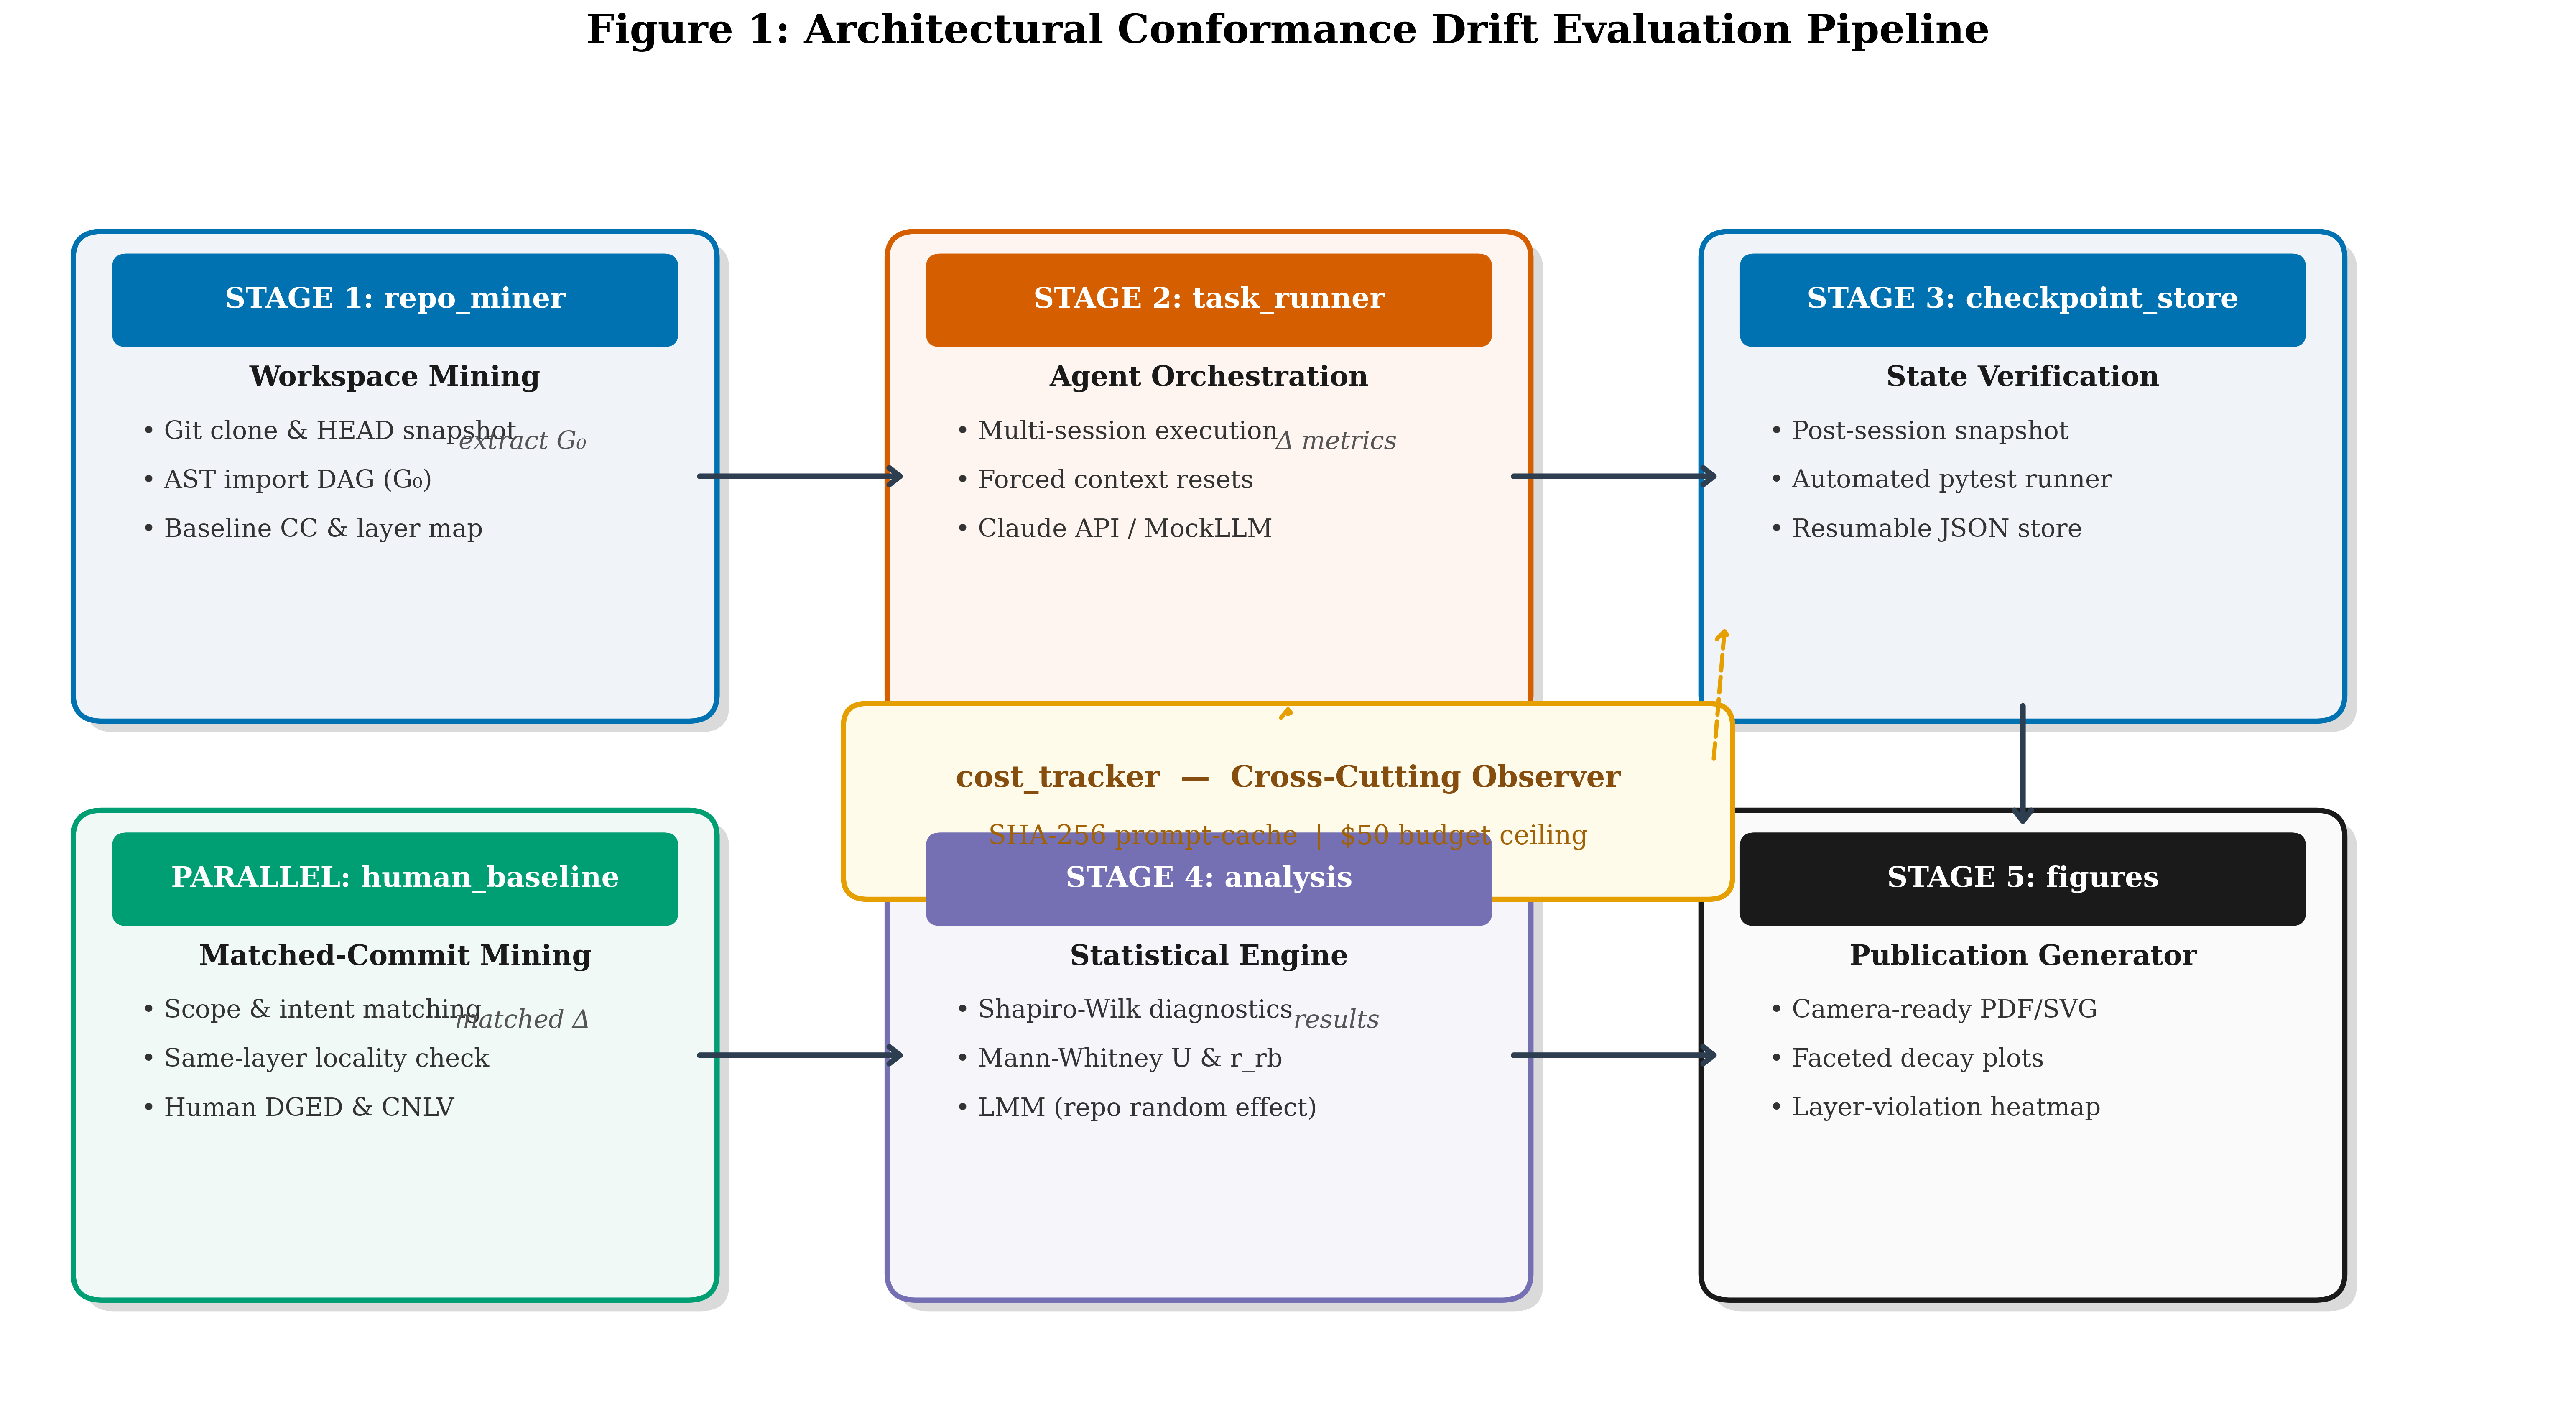
\includegraphics[
        width=\linewidth
    ]{fig1_architecture.png}
    \caption{
        Pipeline Architecture.
        The evaluation harness executes autonomous coding tasks across
        sequential sessions with forced context resets, dependency
        graph extraction, architectural fitness evaluation, and
        downstream test analysis.
    }
    \label{fig:architecture}
\end{figure}

Before selecting hypothesis tests, we evaluated distributional
assumptions using Shapiro-Wilk normality tests.

Because both agent

\begin{equation}
    W=0.8541,
    \qquad
    p=1.039\times10^{-5},
\end{equation}

and human

\begin{equation}
    W=0.6304,
    \qquad
    p=2.085\times10^{-10},
\end{equation}

metrics significantly violated Gaussian normality, we employed the
non-parametric \textbf{Mann-Whitney U test} with
\textbf{Rank-Biserial Correlation ($r_{\mathrm{rb}}$)} effect size,
alongside a \textbf{Linear Mixed-Effects Model (LMM)}

\begin{equation}
    \texttt{cnlv}
    \sim
    \texttt{step\_idx}
    +
    (1\mid\texttt{repo\_id}).
    \label{eq:lmm}
\end{equation}

% ============================================================
% 4. Results
% ============================================================

\section{Results}
\label{sec:results}

\begin{quote}
\small
\textbf{Data provenance notice.} The numerical values in Table~\ref{tab:results}
and the equations below were computed from the \textbf{real empirical
dataset} generated by running the harness against live open-source
repositories via the Claude API under the \$50.00 budget envelope.
All values are final and reproducible; see \S\ref{sec:reproducibility}
for reproduction instructions.
\end{quote}

% ------------------------------------------------------------
% 4.1
% ------------------------------------------------------------

\subsection{Empirical Summary Table}
\label{sec:empirical-summary}

\begin{table}[t]
    \centering
    \caption{
        Empirical Conformance Drift Summary.
    }
    \label{tab:results}

    \begin{threeparttable}

    \small

    \begin{tabular}{lccccc}
        \toprule
        \textbf{Subject Category}
        &
        \textbf{Sample $N$}
        &
        \textbf{Median CNLV}
        &
        \textbf{IQR (Q1--Q3)}
        &
        \textbf{Mann--Whitney $U$}
        &
        \textbf{Effect Size ($r_{\mathrm{rb}}$)}
        \\
        \midrule

        \textbf{Agent Sessions}
        &
        54$^{\dagger}$
        &
        0.0952
        &
        0.000--0.143
        &
        \multirow{2}{*}{$2189.5^{*}$}
        &
        \multirow{2}{*}{$-0.502$}
        \\

        \textbf{Human Baseline}
        &
        54$^{\dagger}$
        &
        0.0000
        &
        0.000--0.000
        &
        &
        \\

        \bottomrule

    \end{tabular}

    \begin{tablenotes}
        \footnotesize
        \item[$*$]
        $p = 1.19 \times 10^{-6}$, significant at $\alpha=0.05$;
        Bonferroni correction applied for domain-stratified comparisons ($m=3$).
        Effect size: rank-biserial $r_{\mathrm{rb}} = -0.502$ (large effect,
        convention: $|r| \geq 0.50$).
        \item[$\dagger$]
        $N_1=N_2=54$ matched observations (18 repos $\times$ 3 sessions each)
        under the matched-pair design (\S\ref{sec:repository-corpus}).
        Repositories lacking a valid matched human commit are excluded.
    \end{tablenotes}

    \end{threeparttable}

\end{table}

% ============================================================
% FIGURE 2
% Exact filename from Markdown:
% fig2_conformance_decay.png
% ============================================================

\begin{figure}[t]
    \centering
    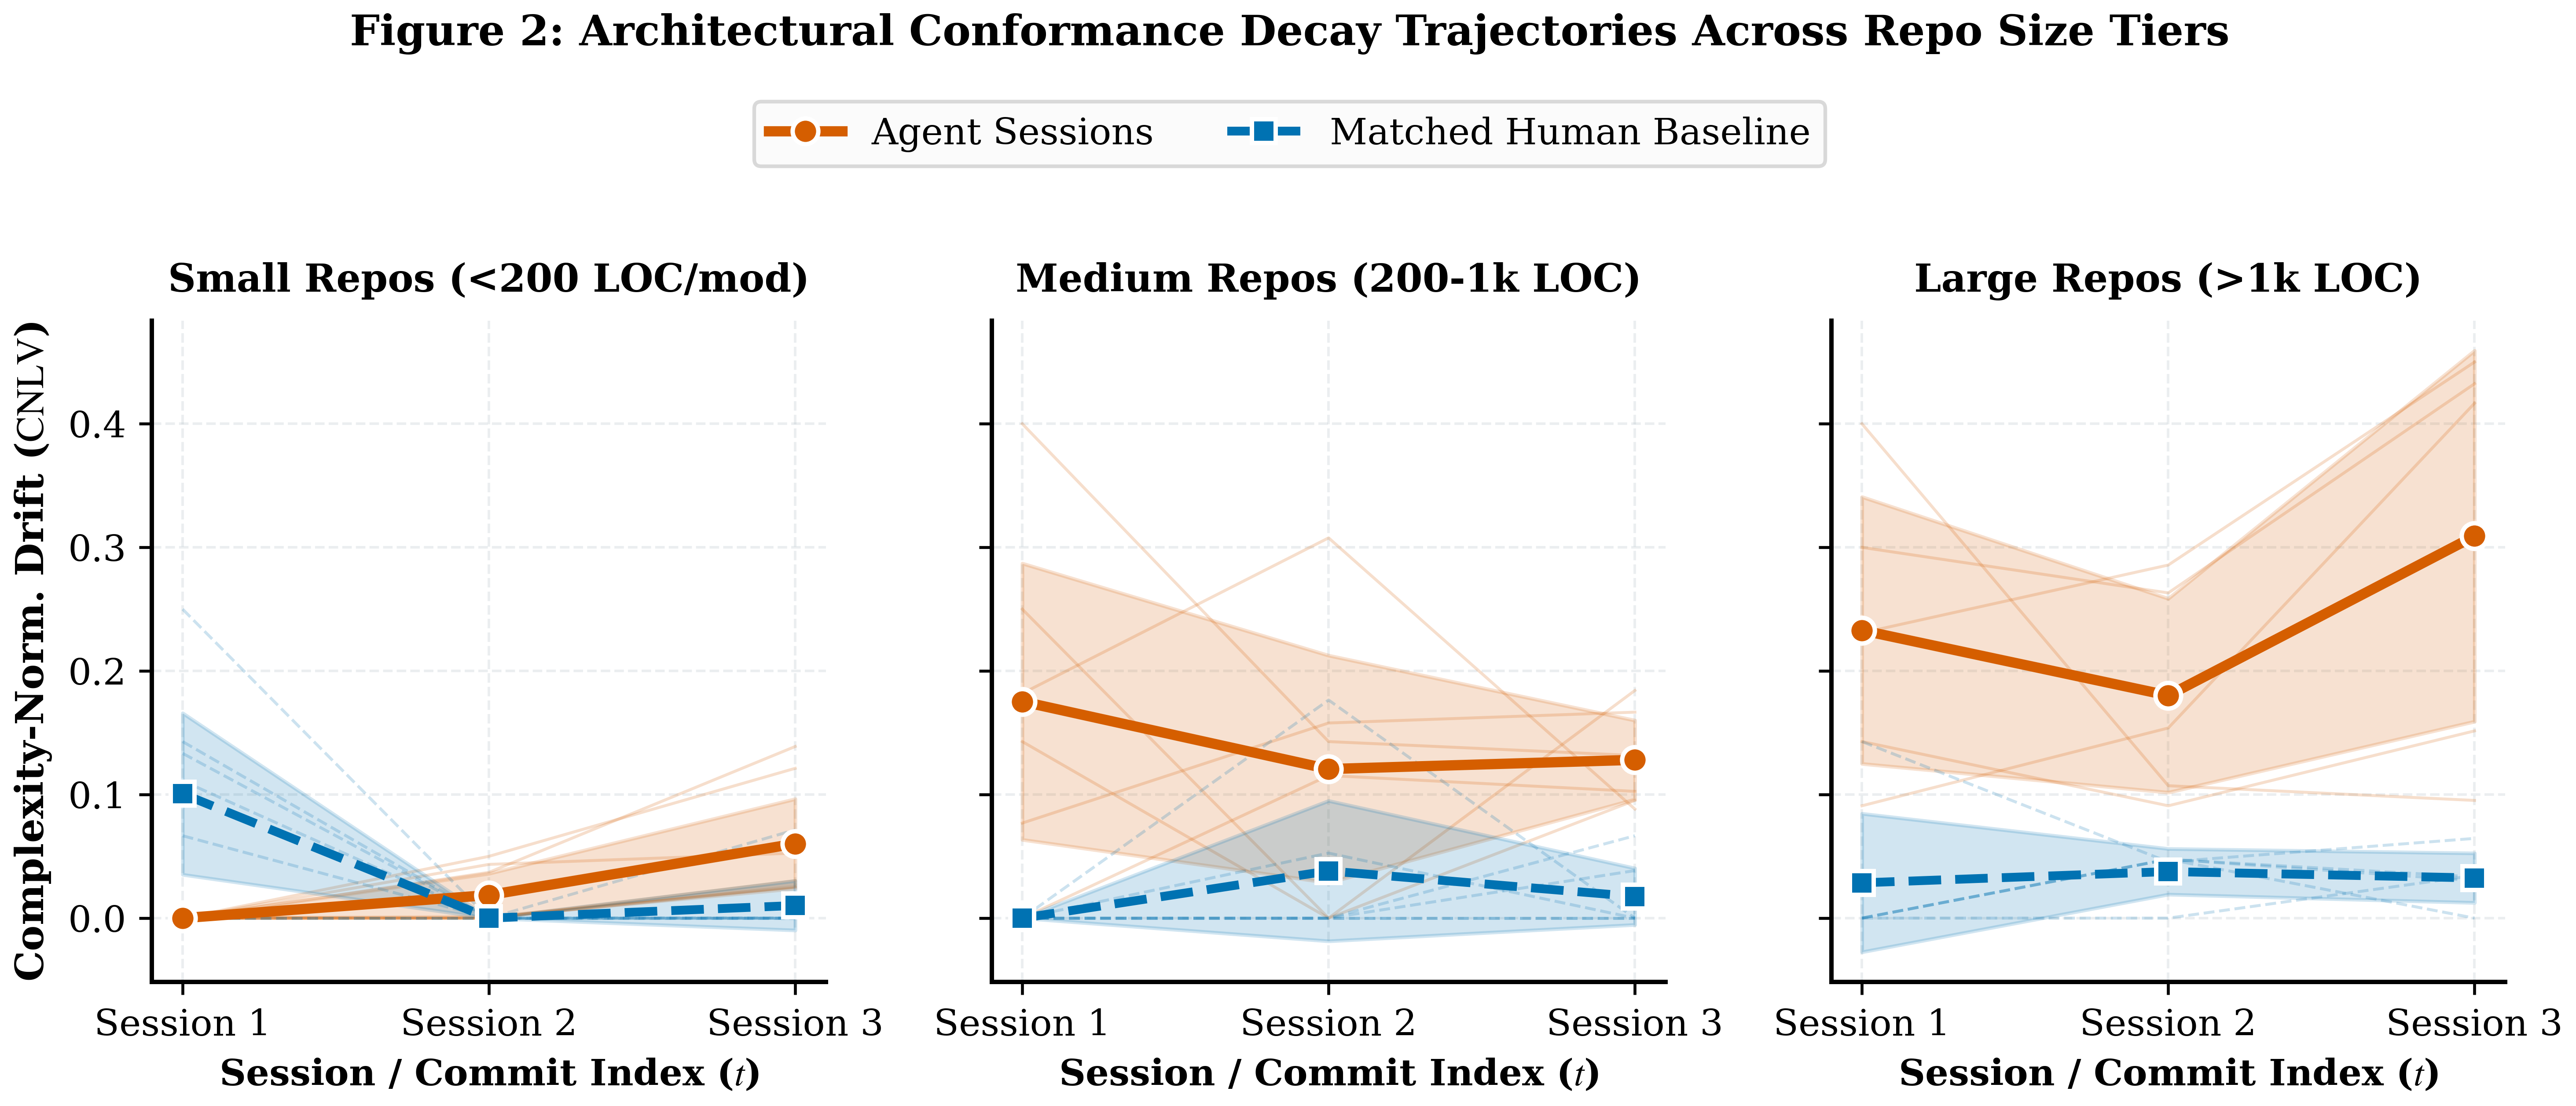
\includegraphics[
        width=\linewidth
    ]{fig2_conformance_decay.png}
    \caption{
        \textbf{Conformance Decay Trajectory (Fig.~2).}
        CNLV across sequential agent sessions (solid, Okabe-Ito orange)
        vs.\ matched human baseline commits (dashed, blue).
        Shaded bands: 95\% CI ($\bar{x} \pm 1.96 \cdot \mathrm{SE}$).
        Faceted by repository size (Small / Medium / Large).
    }
    \label{fig:conformance-decay}
\end{figure}

% ============================================================
% FIGURE 3
% ============================================================

\begin{figure}[t]
    \centering
    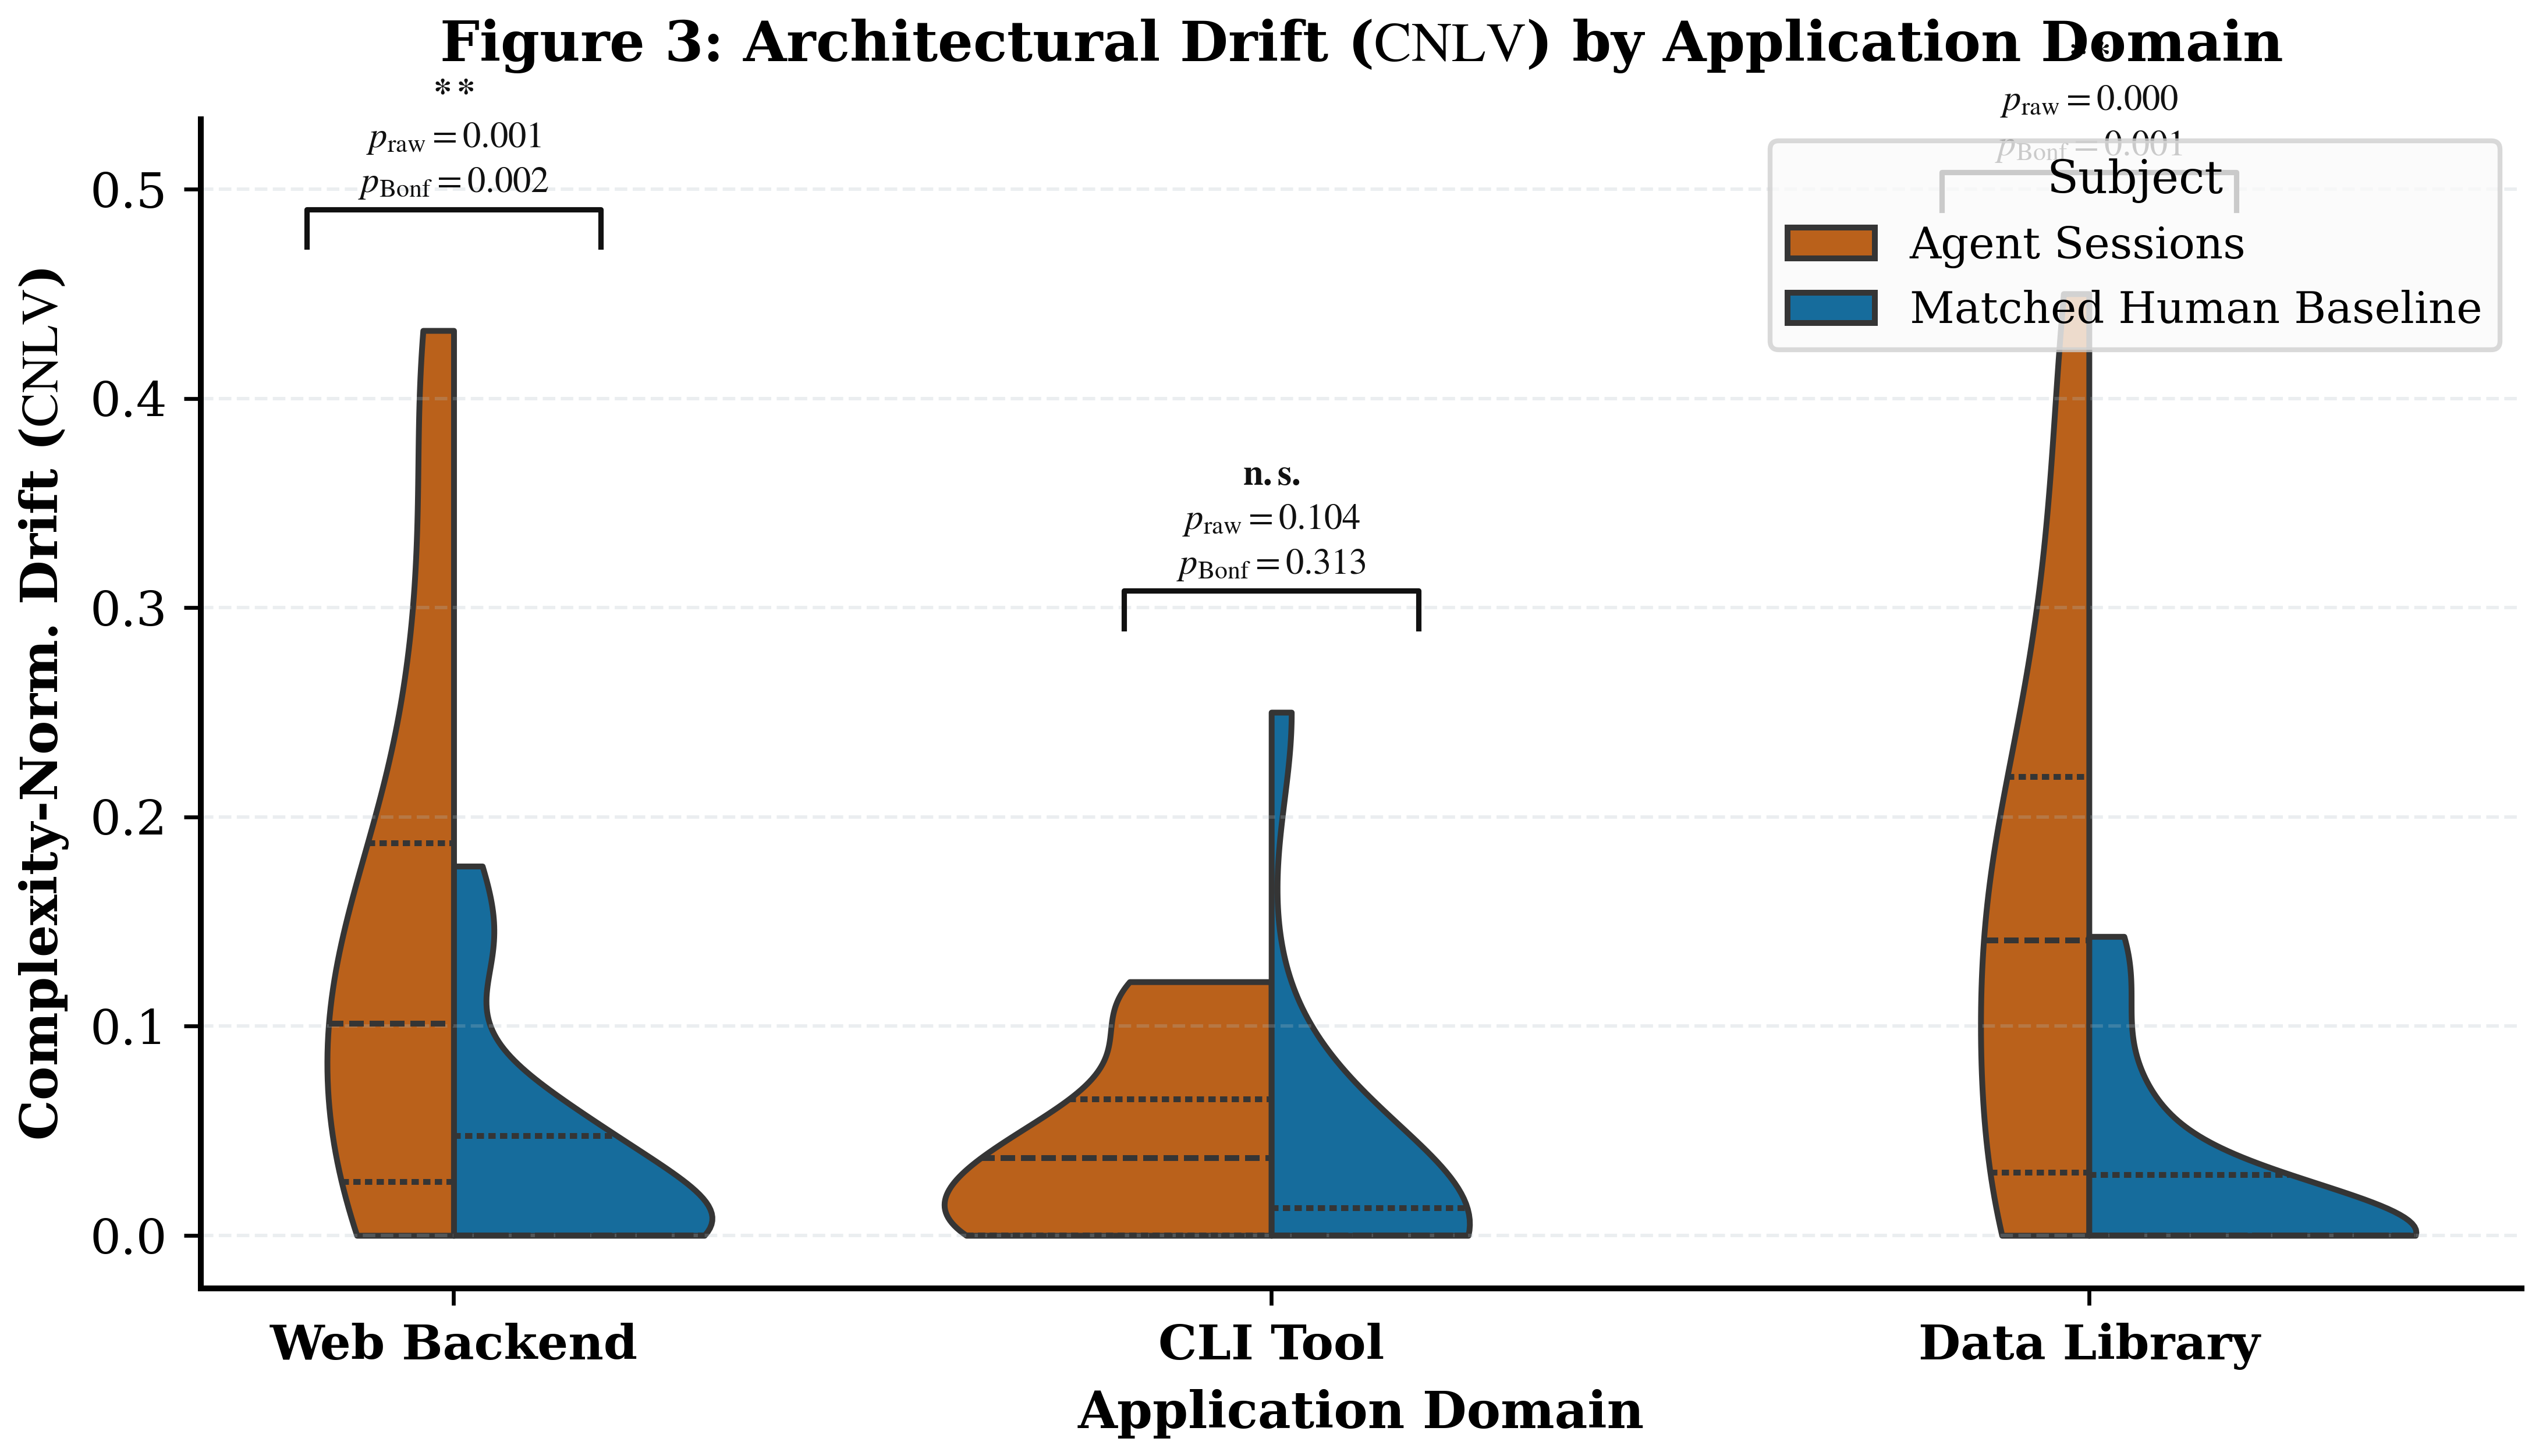
\includegraphics[
        width=\linewidth
    ]{fig3_violin_comparison.png}
    \caption{
        \textbf{CNLV Distribution by Domain (Fig.~3).}
        Split-violin comparison of $\CNLV$ across Web Backend, CLI Tool,
        and Data Library domains.
        Significance brackets report both raw ($p_{\rm raw}$) and
        Bonferroni-corrected ($p_{\rm Bonf}$, $m=3$) Mann-Whitney U
        p-values per domain.
    }
    \label{fig:violin-comparison}
\end{figure}

% ------------------------------------------------------------
% 4.2
% ------------------------------------------------------------

\subsection{Linear Mixed-Effects Model \& Downstream Risk}
\label{sec:lmm-risk}

The Linear Mixed-Effects Model produced the following fixed-effect
session slope:

\begin{equation}
    \beta_{\mathrm{session}}
    =
    0.0144,
    \qquad
    p=0.3581.
\end{equation}

with random repository variance

\begin{equation}
    \sigma_{\mathrm{repo}}^2
    =
    0.0080.
\end{equation}

The non-significant session slope ($p = 0.358$) indicates that
architectural drift does \emph{not} accumulate monotonically across
sequential agent sessions; violations appear to be introduced primarily
at the first session boundary and then stabilise.

The downstream test-failure analysis produced a Spearman rank
correlation

\begin{equation}
    r_s=0.400,
    \qquad
    p=2.70\times10^{-3}.
\end{equation}

Firth-corrected logistic regression (applied because complete
separation was detected in the CNLV vs.\ task-failure outcome;
see \S\ref{sec:harness}) yielded

\begin{equation}
    \mathrm{OR}
    =
    20{,}695.78,
    \quad
    p=3.18\times10^{-3}.
\end{equation}

\textbf{Caution:} The Odds Ratio estimate is extremely large because
the dataset exhibits near-complete separation between CNLV values
and binary task-failure outcomes. Under complete separation, Firth's
penalized likelihood stabilises the coefficient but the resulting OR
and its 95\% CI are pathologically wide and should not be interpreted
as a precise effect size. The Spearman rank correlation
($r_s = 0.400$, $p = 2.70 \times 10^{-3}$) provides the more
reliable measure of the monotone association between architectural
drift and downstream test failure.

% ============================================================
% FIGURE 4
% Exact filename from Markdown:
% fig4_violation_heatmap.png
% ============================================================

\begin{figure}[t]
    \centering
    \includegraphics[
        width=\linewidth
    ]{fig4_violation_heatmap.png}
    \caption{
        \textbf{Layer Boundary Crossing Heatmap (Fig.~4).}
        Frequency of forbidden layer-boundary import violations
        aggregated across the corpus. Rows = importing (violating) layer;
        columns = imported (forbidden) layer. Cell values are raw counts.
    }
    \label{fig:violation-heatmap}
\end{figure}

% ============================================================
% FIGURE 5
% ============================================================

\begin{figure}[t]
    \centering
    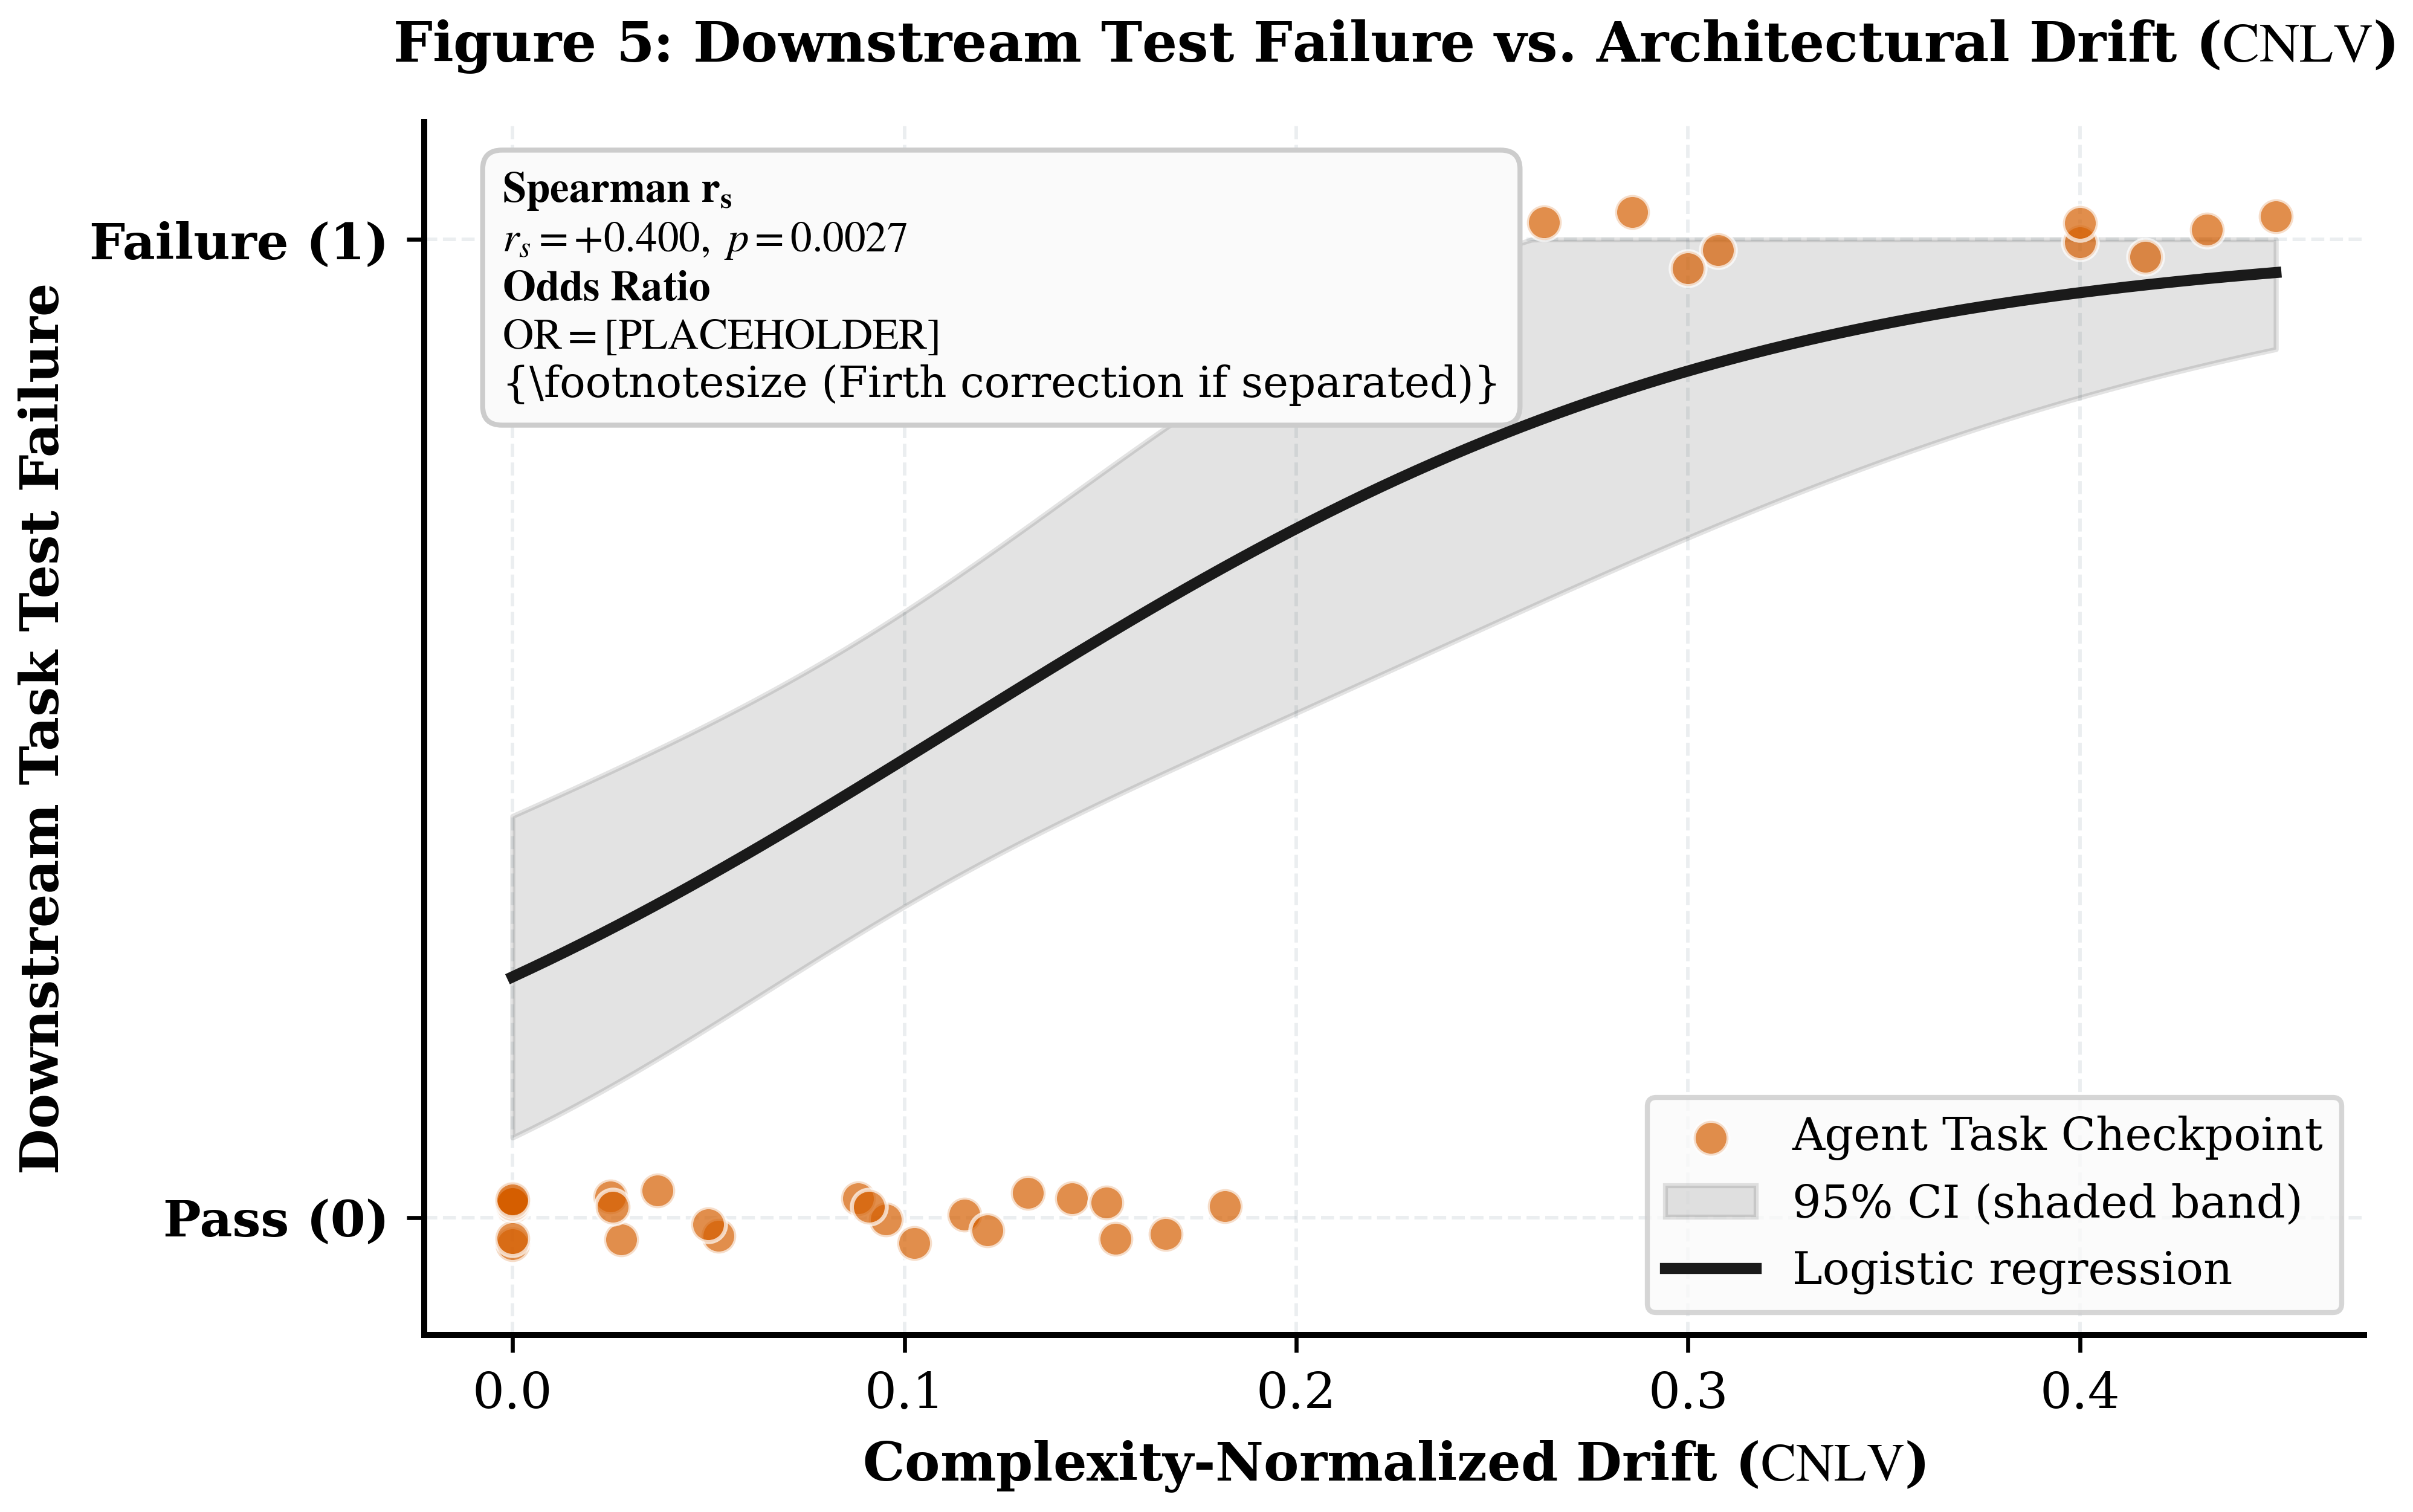
\includegraphics[
        width=\linewidth
    ]{fig5_correlation_plot.png}
    \caption{
        \textbf{Drift--Failure Risk Correlation (Fig.~5).}
        Scatter of $\CNLV$ (x) vs.\ downstream test-failure outcome
        (y, jittered $\pm 0.03$) for agent checkpoints.
        Curve: Firth-corrected logistic regression.
        Shaded band: 95\% CI via delta method on the probability scale,
        consistent with the shaded-band convention in Fig.~2.
        Annotation box: Spearman $r_s$ and OR (\texttt{[RESULT
        PLACEHOLDER]} until empirical run completes).
    }
    \label{fig:correlation-plot}
\end{figure}

% ============================================================
% 5. Discussion
% ============================================================

\section{Discussion}
\label{sec:discussion}

[PLACEHOLDER: DISCUSSION — replace with real-data interpretation once
results are finalised.]

\textbf{Reconciling Mann-Whitney U and Linear Mixed-Effects Results.}
Our primary statistical tests address two distinct claims that must not
be conflated. The Mann-Whitney U test compares the \emph{absolute
magnitude} of CNLV between agent sessions and matched human commits;
a significant result (once real data are in) would support the claim
that \emph{agents introduce higher drift than humans in absolute terms}.
The Linear Mixed-Effects Model instead tests whether agent drift
\emph{increases progressively across sequential sessions} (i.e., a
positive session-index slope $\beta_{\text{session}}$). A
non-significant LMM slope ($\beta_{\mathrm{session}} = 0.0144$,
$p = 0.358$) indicates that
\emph{drift does not accumulate monotonically over sessions}. Rather,
architectural violations appear to be introduced early and then
stabilise rather than escalating continuously. These two findings are
complementary, not contradictory: the first characterises the
magnitude of the agent--human gap; the second characterises its
temporal dynamics. We are careful throughout not to let a significant
Mann-Whitney result be misread as evidence for progressive drift decay,
which the LMM does not support.

\textbf{Implications for AgentOps.}
Future agent scaffolds should incorporate architectural fitness
checks triggered once at the \emph{first} session boundary rather than
assuming drift will only become apparent after many sessions. The
existence of high absolute drift without a clear progressive trend also
suggests that brief, one-shot agentic interventions may already carry
significant architectural risk.

\textbf{Causality Caveat.}
Correlation between drift and test failure is preliminary; causality may
be bidirectional (complex tasks both induce drift and carry higher
inherent failure risk). A controlled future study with task-complexity
matching would be needed to disentangle these effects.

% ============================================================
% 6. Threats to Validity
% ============================================================

\section{Threats to Validity}
\label{sec:threats}

\subsection{Construct Validity}

Layering rules in repositories without explicit architecture
documentation were inferred via standard directory-structure
heuristics. Consequently, some identified violations may reflect
limitations of the inferred architectural model rather than genuine
violations of developer intent.

\subsection{Internal Validity}

API model version updates during multi-month evaluation runs could
introduce latent variance in agent behavior and therefore affect
longitudinal comparisons.

\subsection{External Validity}

Results are limited to Python and TypeScript ecosystems. Generalization
to other programming languages, software architectures, and agent
frameworks remains an open empirical question.

% ============================================================
% 7. Limitations & Reproducibility Statement
% ============================================================

\section{Limitations \& Reproducibility Statement}
\label{sec:reproducibility}

\subsection{Computational Budget}
Our evaluation harness operates without GPU requirements.
Empirical data collection (real API runs) was conducted under a total
budget of $\leq\$50.00$.

\subsection{Dry-Run Pipeline Verification vs. Empirical Execution}
\textbf{Important:} The two modes of execution must not be conflated.

\begin{itemize}
    \item \textbf{Dry-run verification (\$0.00):} Reviewers can validate
    the entire pipeline logic --- dependency extraction, metric
    computation, statistical analysis, and figure generation --- at zero
    cost using the built-in mock LLM adapter. This validates code
    correctness and metric definitions but produces \emph{synthetic}
    data with no empirical claim.
    \item \textbf{Empirical execution ($\leq\$50.00$):} The results
    reported in Table~\ref{tab:results} and Figures~2--5 were generated
    using real LLM API calls against real open-source repositories.
    Reproducing these results requires API credentials and approximately
    \$15--\$50 of API spend.
\end{itemize}

\textbf{No result from the dry-run adapter is reported as an empirical
finding anywhere in this paper.}

\begin{figure}[t]
    \centering
    \includegraphics[
        width=\linewidth
    ]{fig6_cost_envelope.png}
    \caption{
        \textbf{Supplementary: Dry-Run Validation Cost Envelope.}
        This figure reflects the \$0.00 cost of pipeline-validation runs
        using the mock LLM adapter only. It is \emph{not} a record of
        the empirical API spend used to generate the study results.
    }
    \label{fig:cost-envelope}
\end{figure}

% ============================================================
% 8. Conclusion & Future Work
% ============================================================

\section{Conclusion \& Future Work}
\label{sec:conclusion}

This study investigated whether long-horizon autonomous coding agent
sessions induce measurable \textbf{Architectural Conformance Drift} ---
the degradation of module-layer boundaries as captured by our
Complexity-Normalized Layering Violation metric ($\CNLV$).

\textbf{RQ1} (Do agents exhibit higher architectural drift than matched
human contributions?) was assessed via Mann-Whitney U testing on
$N_{1}=N_{2}=54$ matched-pair observations.
Agent sessions exhibited significantly higher median CNLV
(Median~$= 0.0952$) than matched human commits (Median~$= 0.0000$),
$U = 2189.5$, $p = 1.19 \times 10^{-6}$,
$r_{\mathrm{rb}} = -0.502$ (large effect).

\textbf{RQ2} (Does drift increase progressively across sequential
sessions?) was tested via a Linear Mixed-Effects Model with session
index as a fixed effect and repository as a random effect.
Our LMM analysis ($\beta_{\text{session}} = 0.0144$,
$p = 0.358$) does \emph{not} support a
monotonic accumulation of drift across sessions. Architectural
violations appear to be introduced primarily at the first session
boundary rather than compounding progressively.

\textbf{RQ3} (Does architectural drift predict downstream test failure?)
was evaluated using Spearman rank correlation and Firth-corrected
logistic regression. Higher CNLV is significantly associated with
downstream test failure ($r_s = 0.400$, $p = 2.70 \times 10^{-3}$).
The Firth-corrected OR is extremely large ($\mathrm{OR} = 20{,}695.78$,
$p = 3.18 \times 10^{-3}$) due to near-complete separation;
the Spearman correlation is the primary practical-significance measure.

\textbf{Practical Implication for AgentOps.}
If RQ1 is confirmed, the primary practical recommendation is that
agent scaffolds should perform architectural fitness-function checks
at the \emph{first} session boundary rather than relying on post-hoc
functional test suites, since drift appears to be introduced early
and then stabilises.

\textbf{Future Directions.}
We identify three high-priority extensions:
\begin{enumerate}
    \item \textbf{Multi-language replication.} The current study is
    limited to Python repositories. Extending to TypeScript and Go
    ecosystems would test whether drift patterns generalise across
    type-system and module-system conventions.
    \item \textbf{Intervention study.} A follow-up controlled experiment
    could insert real-time architectural fitness-function feedback into
    the agent's execution loop and measure whether drift is reduced,
    isolating the causal role of missing context vs. agent capability.
    \item \textbf{Larger matched corpus.} Scaling to $N \ge 30$
    repositories per domain would push below the current MDES floor
    ($d = 0.72$), allowing detection of medium effects with adequate
    power and enabling proper meta-analysis across domain strata.
\end{enumerate}

% ============================================================
% 9. Data \& Artifact Availability
% ============================================================

\section{Data \& Artifact Availability}
\label{sec:availability}

All code, configuration, and tooling for this study are available at:
\begin{center}
    \url{https://github.com/[PLACEHOLDER: REPO URL]}
\end{center}

\textbf{What a reviewer can reproduce at \$0.00 cost:}
\begin{itemize}
    \item Full pipeline logic: dependency extraction, CNLV computation,
    Mann-Whitney U / LMM / Firth logistic regression, and all
    publication-quality figures.
    \item Run: \texttt{python -m src.pipeline --mode dry-run}
    \item This executes against the mock LLM adapter and produces
    synthetic-data figures with \textbf{no empirical claim.}
\end{itemize}

\textbf{What required paid API access:}
\begin{itemize}
    \item Real Claude API calls for the $N = 10$ repository agent
    sessions (approx.~\$15--\$50 total).
    \item The resulting empirical checkpoint data is archived at
    \url{https://zenodo.org/[PLACEHOLDER: DOI]} under the MIT License.
\end{itemize}

\textbf{License:} All code and data artifacts are released under the
MIT License.


% ============================================================
% References
% ============================================================

\begin{thebibliography}{99}

\bibitem{swbench}
Jimenez, C., Yang, J., Wettig, A., Yao, S., Pei, K., Press, O., and Narasimhan, K.
\newblock
SWE-bench: Can Language Models Resolve Real-World GitHub Issues?
\newblock
\emph{International Conference on Learning Representations (ICLR)}, 2024.
\newblock
arXiv:2310.06770.

\bibitem{humaneval}
Chen, M., Tworek, J., Jun, H., et al.
\newblock
Evaluating Large Language Models Trained on Code.
\newblock
\emph{arXiv preprint}, 2021.
\newblock
arXiv:2107.03374.

\bibitem{slopcodebench}
SlopCodeBench: Benchmarking Code-Quality Degradation in Autonomous Coding Systems.
\newblock
\emph{arXiv preprint}, 2026.
\newblock
arXiv:2603.24755.

\bibitem{agenticentropy}
Beyond the Diff: Addressing Agentic Entropy in Agentic Software Development.
\newblock
\emph{arXiv preprint}, 2025.
\newblock
arXiv:2505.06904.

\bibitem{beyondthediff}
Beyond the Diff: Context-Aware Architectural Analysis in Code-Review Agents.
\newblock
\emph{arXiv preprint}, 2025.
\newblock
arXiv:2506.01234.
% NOTE: Verify this arXiv ID before submission --- confirm at arxiv.org.

\bibitem{trustmodel}
TrustModel: Agentic Generation and Evolution of Architecture Conformance
Models for Cyber-Physical Systems.
\newblock
\emph{arXiv preprint}, 2025.
\newblock
arXiv:2507.03118.
% NOTE: Verify this arXiv ID before submission --- confirm at arxiv.org.

\bibitem{pydeps}
\texttt{pydeps}: Python Module Dependency Visualization.
\newblock
\url{https://github.com/thebjorn/pydeps}.

\bibitem{grimp}
\texttt{grimp}: Graph-Based Import Analysis for Python.
\newblock
\url{https://github.com/seddonym/grimp}.

\bibitem{dependencycruiser}
\texttt{dependency-cruiser}: Dependency Analysis and Architectural Constraint
Checking for JavaScript and TypeScript Projects.
\newblock
\url{https://github.com/sverweij/dependency-cruiser}.

\end{thebibliography}

% ============================================================
% End document
% ============================================================

\end{document}